%%%%%%%%%%%%%%%%%%%%%%%%%%%%%%%%%%%%%%%%%
% Masters/Doctoral Thesis 
% LaTeX Template
% Version 2.5 (27/8/17)
%
% This template was downloaded from:
% http://www.LaTeXTemplates.com
%
% Version 2.x major modifications by:
% Vel (vel@latextemplates.com)
%
% This template is based on a template by:
% Steve Gunn (http://users.ecs.soton.ac.uk/srg/softwaretools/document/templates/)
% Sunil Patel (http://www.sunilpatel.co.uk/thesis-template/)
%
% Template license:
% CC BY-NC-SA 3.0 (http://creativecommons.org/licenses/by-nc-sa/3.0/)
%
%%%%%%%%%%%%%%%%%%%%%%%%%%%%%%%%%%%%%%%%%

%----------------------------------------------------------------------------------------
%	PACKAGES AND OTHER DOCUMENT CONFIGURATIONS
%----------------------------------------------------------------------------------------

\documentclass[
11pt, % The default document font size, options: 10pt, 11pt, 12pt
%oneside, % Two side (alternating margins) by default, uncomment to switch to one side
english,
singlespacing, % Single line spacing, alternatives: onehalfspacing or doublespacing
%draft, % Uncomment to enable draft mode (no pictures, no links, overfull hboxes indicated)
%nolistspacing, % If the document is onehalfspacing or doublespacing, uncomment this to set spacing in lists to single
%liststotoc, % Uncomment to add the list of figures/tables/etc to the table of contents
%toctotoc, % Uncomment to add the main table of contents to the table of contents
%parskip, % Uncomment to add space between paragraphs
%nohyperref, % Uncomment to not load the hyperref package
headsepline, % Uncomment to get a line under the header
%chapterinoneline, % Uncomment to place the chapter title next to the number on one line
%consistentlayout, % Uncomment to match to default the layout of the declaration, abstract...
]{MastersDoctoralThesis} % The class file specifying the document structure

\usepackage[utf8]{inputenc} % Required for inputting international characters
\usepackage[T1]{fontenc} % Output font encoding for international characters
\usepackage{mathpazo} % Use the Palatino font by default
\usepackage[backend=bibtex,style=authoryear,natbib=true]{biblatex}

\addbibresource{../bibliography/sw.bib}

\usepackage[autostyle=true]{csquotes} % Lnguage-dependent quotes in the bibliography

%----------------------------------------------------------------------------------------
%	MARGIN SETTINGS
%----------------------------------------------------------------------------------------

\geometry{
	paper=a4paper, % Change to letterpaper for US letter
	inner=2.5cm, % Inner margin
	outer=3.8cm, % Outer margin
	bindingoffset=.5cm, % Binding offset
	top=1.5cm, % Top margin
	bottom=1.5cm, % Bottom margin
	%showframe, % Uncomment to show how the type block is set on the page
}

%----------------------------------------------------------------------------------------
%	THESIS INFORMATION
%----------------------------------------------------------------------------------------

\thesistitle{Coupling shallow water models with three-dimensional models for the study of fluid-structure interaction problems using the particle finite element method} % print it with \ttitle
\supervisor{Dr. Eugenio \textsc{Oñate}} % print it with \supname
\cosupervisor{Dr. Ignasi \textsc{de-Pouplana}} % print it with \cosupname
\examiner{} % this is not currently used, print it with \examname
\degree{Civil Engineering Ph. D.} % print it with \degreename
\author{Miguel \textsc{Masó}} % print it with \authorname
\addresses{} % this is not currently used, print it with \addressname
\subject{Civil Engineering} % this is not currently used, print it with \subjectname
\keywords{} % this is not currently used, print it with \keywordnames
\university{\href{http://www.upc.edu}{Universitat Politècnica de Catalunya Barcelona Tech}} % print it with \univname
\department{\href{http://www.deca.upc.edu}{Department of Civil and Environmental Engineering}} % print it with \deptname
\group{\href{http://www.cimne.com}{International Centre for Numerical Methods in Engineering}} % print it with \groupname
\faculty{\href{http://www.etseccpb.upc.edu}{Barcelona School of Civil Engineering}} % print it with \facname

\colorlet{wrmBlue}{blue!30!black}
\colorlet{wrmGreem}{green!30!black}
\AtBeginDocument{
\hypersetup{pdftitle=\ttitle} % Set the PDF's title to your title
\hypersetup{pdfauthor=\authorname} % Set the PDF's author to your name
\hypersetup{pdfkeywords=\keywordnames} % Set the PDF's keywords to your keywords
\hypersetup{linkcolor=wrmBlue}
\hypersetup{citecolor=wrmGreen}
}

\begin{document}

\frontmatter % Use roman page numbering style (i, ii, iii, iv...) for the pre-content pages

\pagestyle{plain} % Default to the plain heading style until the thesis style is called for the body content

%----------------------------------------------------------------------------------------
%	TITLE PAGE
%----------------------------------------------------------------------------------------

\begin{titlepage}
\begin{center}

\vspace*{.06\textheight}
{\scshape\LARGE \univname\par}\vspace{1.5cm} % University name
\textsc{\Large Doctoral Thesis}\\[0.5cm] % Thesis type

\HRule \\[0.4cm] % Horizontal line
{\huge \bfseries \ttitle\par}\vspace{0.4cm} % Thesis title
\HRule \\[1.5cm] % Horizontal line
 
\begin{minipage}[t]{0.4\textwidth}
\begin{flushleft} \large
\emph{Author:}\\
\href{http://www.johnsmith.com}{\authorname}
\end{flushleft}
\end{minipage}
\begin{minipage}[t]{0.4\textwidth}
\begin{flushright} \large
\emph{Supervisors:} \\
\href{http://www.jamessmith.com}{\supname} \\
\href{http://www.jamessmith.com}{\cosupname}
\end{flushright}
\end{minipage}\\[.3cm]
 
\vfill

\large \textit{A thesis submitted in fulfillment of the requirements\\ for the degree of \degreename}\\[0.3cm] % University requirement text
\textit{in the}\\[0.3cm]
\groupname\\\deptname\\[.3cm] % Research group name and department name
 
\vfill

{\large \today}\\[1cm]

\includegraphics[width=.5\textwidth]{img/logo_upc.png}
\vfill
\end{center}
\end{titlepage}

%----------------------------------------------------------------------------------------
%	DECLARATION PAGE
%----------------------------------------------------------------------------------------

\begin{declaration}
\addchaptertocentry{\authorshipname} % Add the declaration to the table of contents
\noindent I, \authorname, declare that this thesis titled, \enquote{\ttitle} and the work presented in it are my own. I confirm that:

\begin{itemize} 
\item This work was done wholly or mainly while in candidature for a research degree at this University.
\item Where any part of this thesis has previously been submitted for a degree or any other qualification at this University or any other institution, this has been clearly stated.
\item Where I have consulted the published work of others, this is always clearly attributed.
\item Where I have quoted from the work of others, the source is always given. With the exception of such quotations, this thesis is entirely my own work.
\item I have acknowledged all main sources of help.
\item Where the thesis is based on work done by myself jointly with others, I have made clear exactly what was done by others and what I have contributed myself.\\
\end{itemize}
 
\noindent Signed:\\
\rule[0.5em]{25em}{0.5pt} % This prints a line for the signature
 
\noindent Date:\\
\rule[0.5em]{25em}{0.5pt} % This prints a line to write the date
\end{declaration}

\cleardoublepage

%----------------------------------------------------------------------------------------
%	QUOTATION PAGE
%----------------------------------------------------------------------------------------

% \vspace*{0.2\textheight}

% \noindent\enquote{\itshape Thanks to my solid academic training, today I can write hundreds of words on virtually any topic without possessing a shred of information, which is how I got a good job in journalism.}\bigbreak

% \hfill Dave Barry

%----------------------------------------------------------------------------------------
%	ABSTRACT PAGE
%----------------------------------------------------------------------------------------

\begin{abstract}
\addchaptertocentry{\abstractname} % Add the abstract to the table of contents
The Thesis Abstract is written here (and usually kept to just this page). The page is kept centered vertically so can expand into the blank space above the title too\ldots
\end{abstract}

%----------------------------------------------------------------------------------------
%	ACKNOWLEDGEMENTS
%----------------------------------------------------------------------------------------

\begin{acknowledgements}
\addchaptertocentry{\acknowledgementname} % Add the acknowledgements to the table of contents
The acknowledgments and the people to thank go here, don't forget to include your project advisor\ldots
\end{acknowledgements}

%----------------------------------------------------------------------------------------
%	LIST OF CONTENTS/FIGURES/TABLES PAGES
%----------------------------------------------------------------------------------------

\tableofcontents % Prints the main table of contents

\listoffigures % Prints the list of figures

\listoftables % Prints the list of tables

%----------------------------------------------------------------------------------------
%	ABBREVIATIONS
%----------------------------------------------------------------------------------------

\begin{abbreviations}{ll} % Include a list of abbreviations (a table of two columns)

\textbf{LAH} & \textbf{L}ist \textbf{A}bbreviations \textbf{H}ere\\
\textbf{WSF} & \textbf{W}hat (it) \textbf{S}tands \textbf{F}or\\

\end{abbreviations}

%----------------------------------------------------------------------------------------
%	PHYSICAL CONSTANTS/OTHER DEFINITIONS
%----------------------------------------------------------------------------------------

\begin{constants}{lr@{${}={}$}l} % The list of physical constants is a three column table

% The \SI{}{} command is provided by the siunitx package, see its documentation for instructions on how to use it

Speed of Light & $c_{0}$ & \SI{2.99792458e8}{\meter\per\second} (exact)\\
%Constant Name & $Symbol$ & $Constant Value$ with units\\

\end{constants}

%----------------------------------------------------------------------------------------
%	SYMBOLS
%----------------------------------------------------------------------------------------

\begin{symbols}{lll} % Include a list of Symbols (a three column table)

$a$ & distance & \si{\meter} \\
$P$ & power & \si{\watt} (\si{\joule\per\second}) \\
%Symbol & Name & Unit \\

\addlinespace % Gap to separate the Roman symbols from the Greek

$\omega$ & angular frequency & \si{\radian} \\

\end{symbols}

%----------------------------------------------------------------------------------------
%	DEDICATION
%----------------------------------------------------------------------------------------

\dedicatory{For/Dedicated to/To my\ldots} 

%----------------------------------------------------------------------------------------
%	THESIS CONTENT - CHAPTERS
%----------------------------------------------------------------------------------------

\mainmatter % Begin numeric (1,2,3...) page numbering

\pagestyle{thesis} % Return the page headers back to the "thesis" style

% Include the chapters of the thesis as separate files from the chapters folder


\chapter{Introduction}
\label{chapter_introduction}



%%%%%%%%%%%%%%%%%%%%%%%%%%%%%%%%%%%%%%%%%%%%%%%%%%%%%%%%%%%%

\section{Overview}


The continued increase of computing resources available for scientific and industrial research has motivated the simulation of complex flows. Several attempts have been done in order to fully simulate water-related hazards, from the its generation to its interaction with structures.

Usually, water-related hazards involve floods, which are complex natural phenomena with a great assortment of causes and a huge casuistic depending on the land characteristics or the climatic conditions. Preventing floods is still a great challenge due to uncertainty of climatic conditions and complexity of modeling land, usually defined by a great number of variables and parameters.

Furthermore, it is possible to identify several scales, local and global, whereas the local scale requires a high fidelity simulation. The identification of different levels of resolution makes the global simulation of these phenomena still unaffordable. From one side, the event generation can be global or local. If it is local, a \emph{Fluid-Structure Interaction} (FSI) simulation may be needed. The propagation of the event usually allows to assume several simplifications, corresponding to the large scale field. Finally, the interaction with structures is strictly a local scale.

\emph{Landslide-Generated Waves} (LGW) are an example of water-related natural hazards. Those events are originated when a landslide impacts a water reservoir and produces large-amplitude waves. LGW events can have devastating effects on the coastal areas of water basins, such as lakes, fjords and artificial reservoirs. Accurate modeling and prediction of LGWs are of key importance to reduce their catastrophic effects. Both experimental and numerical studies have been greatly contributed to the enhancement of the forecasting capabilities against these natural hazards. In that case, both the generation of the impulse wave and the interaction with structures require a local-scale resolution.

The direct simulation of all the scenario with a local scale resolution is computationally highly demanding and it can be unaffordable as long as the size of the scenario increases. This fact leads to the consideration of alternative strategies combining the numerical simulation of the large and local scale in a staggered frame. Figure \ref{space_time_staggered_approach} shows a conceptual identification of the different scales and the possible approaches. The computational cost is proportional to the area enclosed by the space-time domain and proportional to the efficiency of each solver. In Figure \ref{space_time_staggered_approach} the local-scale resolution is identified with a \emph{Near Field Solver} (NFS) and the large-scale resolution is identified with a \emph{Far Field Solver} (FFS).

The staggered approach, apart from being computationally more efficient, allows to decouple the uncertainty related to the generation from the FSI simulation. In addition, the staggered approach allows to concentrate the computational resources only where it is needed, thus having a more intelligent level of accuracy.


\begin{figure}
    \centering
    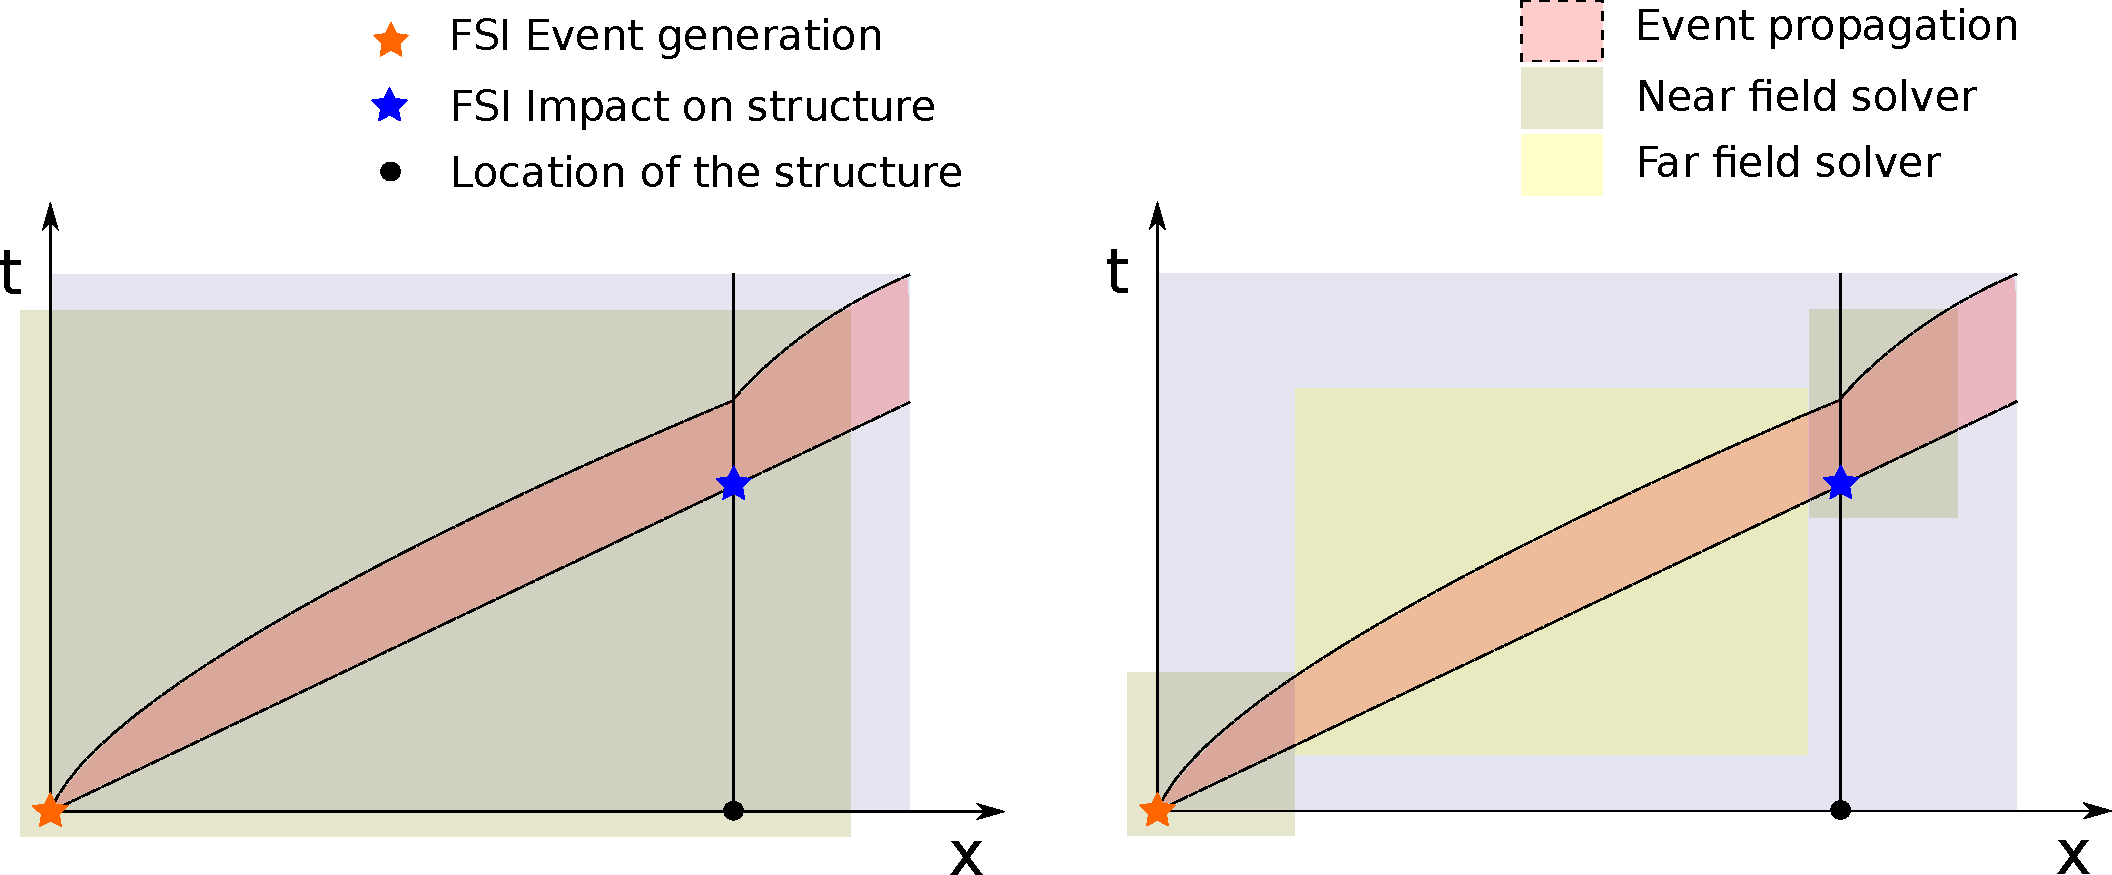
\includegraphics[width=\textwidth]{img/coupling/space_time}
    \caption{Propagation path of the event and possible computational approaches. Left: Brute force approach. Right: Staggered approach.}
    \label{space_time_staggered_approach}
\end{figure}


The main aspects that have been explored in this thesis are the numerical approximation of the FFS and the coupling strategy of the proposed FFS and an existing NFS. Special attention have been paid to the convergence and stability properties of the FFS aimed to solve the large scale.




%%%%%%%%%%%%%%%%%%%%%%%%%%%%%%%%%%%%%%%%%%%%%%%%%%%%%%%%%%%%

\section{Objectives and outline}


The work developed within the framework of this thesis can be enclosed in the global objective of investigating Finite Element formulations applied to large-scale water-related hazards. In particular, the analyzed methods have to be capable of reproducing local-scale effects around structures of interest and accurately model the large-scale propagation. This requirement lead to the analysis of the Finite Element Method for solving the Navier-Stokes equations on local scales and solving the shallow water equations on large scales.

The Navier-Stokes equations are typically solved using the finite element method, while the shallow water equations are often solved using the finite volume method.
Since we are interested in solving within the same framework the global simulation, a previous investigation on stabilized finite elements for the shallow water equations is presented.


This thesis is structured in 6 chapters, including the present introduction and a bibliographic revision. The bibliographic revision is specially extensive for the shallow water equations.
Chapter \ref{equations} presents a review of the governing equations which will be solved in the latter chapters.

Chapter \ref{eulerian_sw} is dedicated to the Finite Element Method applied to the shallow water equations. Stabilized formulations and quasi-monotonic formulations are presented.
Part of the developments of the numerical methods for the shallow water equations are moved to appendices \ref{lagrangian_sw} and \ref{mesh_refinement}, where the particle methods and mesh refinement are explored.
%This family of methods present some interesting properties, such as the natural approximation of the shoreline. The inconvenient of the Particle methods is the lack of robustness for all the possible flow regimes.

An extension of the shallow water equations to wave propagation on intermediate and deep water is presented in chapter \ref{eulerian_bsq}. These equations are known as the Boussinesq equations. The strategies developed in the previous chapter are applied to the Boussinesq equations, however, additional requirements must be fulfilled in order to ensure stability and accuracy. This chapter is of crucial importance in order to analyze impulse waves in the context of water-related hazards.

Chapter \ref{coupling} is devoted to the coupling strategies between the shallow water approximations --specially the Boussinesq equations-- and the fully resolved methods. An example of coupling for landslide long wave generation is provided.

Finally, the thesis is closed with some conclusions and possible further research lines in chapter \ref{conclusions}.


%%%%%%%%%%%%%%%%%%%%%%%%%%%%%%%%%%%%%%%%%%%%%%%%%%%%%%%%%%%%

\section{Research dissemination}


Some of the developments if this thesis have been published in the format of articles in peer reviewed journals. Since the research has advanced gradually, the articles are related to a chapter, but there are some differences, which can be big.
The chapters are more extensive than the articles and some parts of the articles are omitted to avoid repetitions.
There is also not the same sequence between the publication date and the chapter order.
On the other hand, since the notation is introduced gradually, it has been unified in the thesis and may be slightly different from the articles and this document.

\paragraph{Chapter \ref{eulerian_sw}} \fullcite{maso2022}
\paragraph{Chapter \ref{coupling}} \fullcite{maso2022b}
\paragraph{Appendix \ref{lagrangian_sw}} \fullcite{puigferrat2021}
\\

In addition, the content of the chapters has been also disseminated in the form of oral presentations in scientific conferences and congresses:

\paragraph{Chapter \ref{coupling}} WCM
\paragraph{Chapter \ref{coupling}} CMN
\paragraph{Chapter \ref{coupling}} Franci
\paragraph{Appendix \ref{lagrangian_sw}} Particles 2019

%%%%%%%%%%%%%%%%%%%%%%%%%%%%%%%%%%%%%%%%%%%%%%%%%%%%%%%%%%%%


\section{State of the art}
\label{state_art}


In this chapter a bibliographic revision of the methods employed to solve free surface flows problems is presented.
The analysis of the numerical methods for the shallow water equations is more extensive than the review for the Navier-Stokes equations, since this thesis presents some advances in the numerical simulation of the shallow water equations.



\subsection{Numerical methods for the Navier-Stokes model}

% \subsubsection{Overview}

% \subsubsection{Particle methods}



\subsection{Numerical methods for the shallow water models}


\subsubsection{Overview}

The computation of the dry-wet interface of the shallow water equations is a challenging problem. Due to the hyperbolic character of the equations the water height requires positivity ($h>0$) and oscillations can trigger global failure of the system. Löhner \cite{lohner2008} made a review of possible approximation methods to solve fluid dynamics. Being $u^h = N^i\hat{u}_i$ ($i=1,2,\dots,m$) an approximation of the solution $u$, the weighted residual is defined as

\begin{equation}
\int_{\Omega} W^ir(u^h)d\Omega = 0
\end{equation}

\begin{table}
\centering
\begin{tabular}{|l|c|c|}
\hline
 & $N^i$ & $W^i$ \\ \hline
Finite differences (FD)         & polynomial & $\delta(x_i)$ \\ \hline
Finite volumes (FV)             & polynomial & $1 \ \text{if} \ x\in\Omega_{el}$ \\ \hline
Galerkin finite elements (FEM)  & polynomial & $N^i$ \\ \hline
Discontinuous Galerkin (DG)     & polynomial & $N^i \ \text{if} \ x\in\Omega_{el}$ \\ \hline
\end{tabular}
\caption{Possible choices of trial and test functions $N^i$ and $W^i$}
\label{possible_trial_functions}
\end{table}

In table \ref{possible_trial_functions} there are a set of possible trial and test functions and the resulting approximation method. In the recent decades a new family of finite elements have been developed which are known as the discontinuous Galerkin (DG). We are interested on the implementation of \emph{continuous Galerkin finite elements} in KratosMultiphysics.


\subsubsection{Stabilized methods}



\subsubsection{Monotonicity preserving finite elements}

Following Löhner review, there are three classical approaches: stabilized finite elements \cite{lohner2008}, flux corrected transport (FCT) \cite{lohner2008ch9} and edge based finite elements \cite{lohner2008ch10}.

\paragraph*{Stabilized FEM} Streamline-diffusion methods like SUPG are stable but not
monotonicity preserving. However, Badia and Hierro presented a monotonicity preserving stabilized finite element for hyperbolic equations \cite{badia2014}.

\paragraph*{FCT} The way to circumvent the Godunov barrier theorem \cite{godunov1959} is to develop a nonlinear scheme. FCT uses a low order (LO) monotonic scheme with a lot of diffusion and a high order (HO) oscillatory scheme. The process of combining the two schemes is called limiting:

\begin{equation}
\phi^{n+1} = \phi^n + c_e\Delta \phi_H + (1-c_e)\Delta \phi_L
\end{equation}

\paragraph*{Edge based} The edge based structure is an efficient way to assemble the system matrix which resort to a
finite volume approximation of convective terms. If it is assumed that the fluxes of the variables are constant along the edges, a discontinuity will occur at the edge midpoint. Then, one can replace the Galerkin flux by a Riemann flux and obtain a total variational diminishing scheme (TVD).


% \subsubsection{Particle methods}



\subsection{Coupling strategies}





\chapter{Governing equations for free surface flows}
\label{equations}



%Before introducing the review of the numerical methods, the governing equations will be presented.
%The following sections are devoted for the numerical methods.
%The last section is about the coupling algorithms.



%\section{Free surface flows}


Water related natural hazards usually involve free surface flows.
This property allows to assume some simplifications, specially at the large scale.
For this reason, the general case describing the fluid motion is presented first, the Navier-Stokes equations.
Then, some simplifications for the free surface flows are made, yielding the shallow water equations. Different assumptions for the depth integrated models will provide different sets of equations and its range of applicability as well as physical properties will be explained.




\section{Navier-Stokes equations}
\label{equations_ns}


The motion of a fluid is described by the Navier-Stokes equations. The case of a free surface flow is described by that equations and the free surface is located where the densities or the fluid properties are discontinuous. In general, an air-water interface is assumed but some natural phenomena may include a more complex configuration, such as debris flow-air-water interfaces. All this continuous media can be considered isotermal and incompressible, and the standard formulation of the Navier-Stokes equations can be used.

The problem consists in the incompressible Navier-Stokes equations in a time interval $(0, t_f)$ and in a spatial domain $\Omega \in \mathbb{R}^{n_d}$, being $n_d$ the number of space dimensions, $3$ unless otherwise stated. Let $t$ be a certain time instant in the temporal domain $(0, t_f)$ and $\mathbf{x}$ a given point in the spatial domain $\Omega$. The balance equations for the momentum and mass are written in the following form:
\begin{subequations} \label{NS}
    \begin{align} \label{NS1}
        \pder{u_i}{t} + u_j \pder{u_i}{x_i} + \frac{1}{\rho} \pder{p}{x_i} +
            \frac{1}{\rho} \pder{}{x_i} \tau_{ij} &= f_i \\ \label{NS2}
        \pder{u_i}{x_i} &= 0
    \end{align}
\end{subequations}
With the appropriate initial and boundary conditions. Let $\Gamma$ be the boundary of the domain $\Omega$ and $\mathbf{n}$ the unit outward normal on $\Gamma$. Dirichlet and Neumann boundary conditions are considered, $\Gamma_D$ and $\Gamma_N$ respectively, such that $\Gamma_D \cup \Gamma_N = \Gamma$.
The usual summation convention is used if there is index repetition.
$\rho$ is the fluid density, $p$ is the pressure, $\mathbf{u}$ is the velocity, $\bm{\tau}$ is the viscous stresses tensor and $\mathbf{f}$ is the body forces vector.




%%%%%%%%%%%%%%%%%%%%%%%%%%%%%%%%%%%%%%%%
%%%%%%%%%%%%%%%%%%%%%%%%%%%%%%%%%%%%%%%%
%%%%%%%%%%%%%%%%%%%%%%%%%%%%%%%%%%%%%%%%




\section{Shallow water equations}
\label{equations_sw}


The flow of water in shallow layers occurs in a wide range of situations, such as coastal dynamics and hydraulics. In these free surface flows in relatively thin layers compared to the characteristic horizontal length, the horizontal velocities are of primary importance. Under that circumstances, the problem can be reasonably approximated the horizontal plane.

The shallow water equations are the result of integrating vertically the Navier-Stokes equations, assuming incompressibility, small vertical velocity and negligible vertical acceleration \cite{abbott1979,zien3}. The assumptions over the vertical velocity and its acceleration are equivalent to hydrostatic pressure, in fact, the vertical component of the momentum equation (\ref{NS1}) is reduced to
\begin{equation} \label{SW_hydrostatic_pressure}
    \frac{1}{\rho}\pder{p}{x_3} + g = 0
\end{equation}

After substitution of the hydrostatic pressure assumption \ref{SW_hydrostatic_pressure} into the mass conservation \ref{NS2}, the governing equations are integrated from the bottom $z$ to the free surface $\eta$. The problem is closed by adding two kinematic boundary conditions at the bottom and the free surface:
\begin{equation}
    u_3(\eta) = \frac{D\eta}{Dt} \ , \quad u_3(z) = \frac{Dz}{Dt}
\end{equation}


The governing equations are expressed in terms of a new set of primary variables: the water depth and the horizontal flow rate. The water depth is defined by the integration limits, $h = z + \eta$ and the averaged horizontal flow rate $\mathbf{q}$ is defined by the following integrated value,
\begin{equation} \label{SW_averaged_momentum}
    \mathbf{q} = \int_z^\eta \mathbf{u}\,dx_3
\end{equation}
To avoid introducing extra notation, in a shallow water context, $\mathbf{u}$ refers to the averaged horizontal velocities. In that case, the expression \ref{SW_averaged_momentum} can be reduced to a compact form as $\mathbf{q} = h\mathbf{u}$.


Here we find that the resulting equations are written in the same form as the Euler conservation equations. In spite the equations present some similarities to the compressible flow, the shallow water equations are describing a purely incompressible fluid: the variable water depth is playing the role of the variable pressure in compressible fluids. The equations read
%The equations governing mass and momentum conservation can be written in conservative form with water depth $h$ and specific discharge $\mathbf{q}=(h\mathbf{u})$ as follows,
\begin{equation} \label{general_sw}
\pder{\bm{\phi}}{t} + \pder{\mathbf{F}_i}{x_i} + \pder{\mathbf{G}_i}{x_i} + \mathbf{Q} = \mathbf{0} \qquad \text{for} \enspace i=1,2
\end{equation}
with

\begin{subequations}\label{variables_and_fluxes}
\allowdisplaybreaks
\begin{align}
\bm{\phi} &= \left\{
    \begin{array}{c}
        hu_1 \\
        hu_2 \\
        h
    \end{array}\right\} \\
\mathbf{F}_i &= \left\{
    \begin{array}{c}
        hu_1u_i + \delta_{1i}\frac{1}{2}g(h^2 - z^2) \\ [5pt]
        hu_2u_i + \delta_{2i}\frac{1}{2}g(h^2 - z^2) \\ [5pt]
        hu_i
    \end{array}\right\} \\
\mathbf{G}_i &= \left\{
    \begin{array}{c}
        -(h/\rho) \bar{\tau}_{1i} \\ [5pt]
        -(h/\rho) \bar{\tau}_{2i} \\ [5pt]
        0
    \end{array}\right\} \\
\mathbf{Q} &= \left\{
    \begin{array}{c}
        \displaystyle -g(h-z)\pder{z}{x_1} + \frac{h}{\rho}\pder{p_a}{x_1}
        - \frac{1}{\rho}\tau^s_{31} + \frac{1}{\rho}\tau^b_{31} \\ [10pt]
        \displaystyle -g(h-z)\pder{z}{x_2} + \frac{h}{\rho}\pder{p_a}{x_2}
        - \frac{1}{\rho}\tau^s_{32} + \frac{1}{\rho}\tau^b_{32} \\ [10pt]
        r
    \end{array}\right\}
\end{align}
\end{subequations}
where $\bm{\phi}$ is the vector of conserved variables, $\mathbf{F}_i$ is the vector of convective fluxes, $\mathbf{G}_i$ is the vector of viscous fluxes and $\mathbf{Q}$ is the vector source terms. In Figure \ref{diagram} there is a representation of the variables and the notation. The coordinates are denoted with the index notation $x_i$. Since this formulation is defined in a two dimensional space ($n_d=2$), in the following we will consider $i=1,2$.
$\delta_{ij}$ is the Kronecker delta. The topography is expressed with the variable $z$ and the free surface elevation is expressed in terms of the topography and the total depth, $\eta = z + h$. $\bar{\tau}_{ij}$ are the averaged horizontal stresses, and $\tau^b_{3i}$ and $\tau^s_{3i}$ denote the bottom and surface friction stresses respectively. Finally, $r$ is the rain source term and $p_a$ is the atmospheric pressure.


\begin{figure}
    \centering
    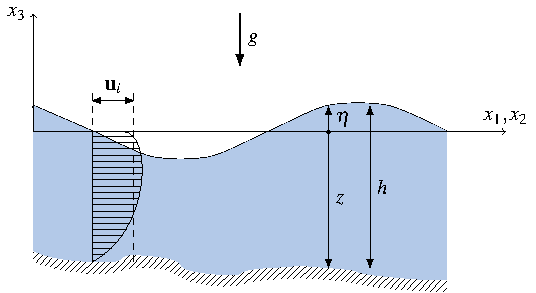
\includegraphics[width=.8\textwidth]{img/eq/diagram.pdf}
    \caption{Diagram and notation for the balance equations (\ref{general_sw}) and (\ref{variables_and_fluxes})}
    \label{diagram}
\end{figure}



Usually, the bottom friction $\tau^b_{3i}$ from (\ref{variables_and_fluxes}) is modelled with a semi-empirical formula, such as the Chezy or the Manning formula. The Manning formula generalized for two dimensions is as follows:
\begin{equation}
\frac{\tau^b_{3i}}{\rho} = -gn^2\frac{\abs{\mathbf{q}}\mathbf{q}}{h^{\sfrac{7}{3}}}
\end{equation}
where $n$ is the Manning roughness coefficient. It defines the resistance to flow by the roughness of the bottom or other macroscopic factors and it is determined empirically. In practice, the Manning coefficient varies from $0.009$ for a very smooth bed (concrete) to $0.05$ for a rough bed (rocks) \cite{chow1988}.


The averaged horizontal stresses are calculated from the combination of the molecular stresses and the Reynolds stresses as follows
\begin{equation} \label{stresses}
\frac{\bar{\tau}_{ij}}{\rho} = (\nu + \nu_t)\left(
    \pder{u_i}{x_j} + \pder{u_j}{x_i} -\frac{2}{3}\delta_{ij}\pder{u_k}{x_k} \right)
\end{equation}
where $\nu$ is the kinematic viscosity and $\nu_t$ is the turbulent kinematic viscosity. When any model of turbulence is considered, the turbulent stresses can be considered as included in the bottom friction with the Manning formula \cite{blade2005}. In this work, the turbulent stresses will be neglected.



Returning again to the equations structure, the Euler conservation laws define two eigenvalues fo the one-dimensional case: $\lambda = u \pm c$. Where $u$ is the modulus of the velocity and $c=\sqrt{gh}$ is the phase speed or wave speed.
In the case of positive eigenvalues, the flux is supercritical, this means that the information travels in one direction, the velocity is higher than the phase speed. When the eigenvalues are of different sign, the flow is subcritical. If one of the eigenvalues is zero, the flow becomes critical and is unstable, so it will derive to a stable solution, sub or supercritical.

For the two dimensional case, does not exist a unique decomposition and this is known as amplitude dispersion. This means there is not an unique direction of propagation. The projection to the velocity direction -the main direction- will provide the eigenvalues $\lambda_1 = u - c$, $\lambda_2 = u$ and $\lambda_3 = u + c$.



%%%%%%%%%%%%%%%%%%%%%%%%%%%%%%%%%%%%%%%%
%%%%%%%%%%%%%%%%%%%%%%%%%%%%%%%%%%%%%%%%



\subsection{Boundary conditions}
\label{equations_sw_bc}


The problem is closed with appropriate boundary conditions: an initial condition
\begin{equation}
\bm{\phi}(t=t_0) = \bm{\phi}_0
\end{equation}
where $\bm{\phi}_0$ are the initial water height and specific discharge. And boundary conditions at $\Gamma$, being $\Gamma$ the boundary of the domain $\Omega$. The boundary $\Gamma$ is split into three subdomains, $\Gamma_I$, $\Gamma_O$ and $\Gamma_S$: inflow, outflow and solid.
\paragraph{Inflow boundary} the flow rate is known
\begin{equation*}
    \mathbf{q} = \mathbf{q}_{in} \quad \text{in} \quad \Gamma_{in}
\end{equation*}
If the inflow is supercritical, the water depth is also specified
\begin{equation*}
    \left.\begin{matrix}
    \mathbf{q} = \mathbf{q}_{in} \\
    h = h_{in}
    \end{matrix}\right\}
    \quad \text{in} \quad \Gamma_{in}
\end{equation*}


\paragraph{Outflow boundary} The water depth is known
\begin{equation*}
    h = h_{out} \quad \text{in} \quad \Gamma_{out}
\end{equation*}
if the outflow is supercritical, no conditions have to be imposed.


\paragraph{Solid boundary} slip or no slip condition can be imposed
\begin{equation*}
    \mathbf{q} \cdot \mathbf{n} = 0 \quad \text{or} \quad \mathbf{q} = \mathbf{0} \quad \text{in} \quad \Gamma_{solid}
\end{equation*}



%%%%%%%%%%%%%%%%%%%%%%%%%%%%%%%%%%%%%%%%
%%%%%%%%%%%%%%%%%%%%%%%%%%%%%%%%%%%%%%%%



\subsection{Linearization}

Usually, in the numerical study of the conservation equations, them are expressed in a quasi-linear form. The balance equation (\ref{general_sw}) can be linearized as follows


\begin{equation} \label{general_sw_lin}
\pder{\bm{\phi}}{t} + \mathbf{A}_i\pder{\bm{\phi}}{x_i}
 - \pder{}{x_{i}}\left(\mathbf{K}_{ij}\pder{\bm{\phi}}{x_j}\right) + \mathbf{S}\bm{\phi} + \mathbf{b}_i\pder{z}{x_i} = 0
\end{equation}
where the matrices $\mathbf{A}_i$ and $\mathbf{K}_{ij}$ are the linearization matrices of the convective fluxes and the diffusive fluxes respectively. The convective matrices $\mathbf{A}_i$ are obtained after applying the chain rule to the vector of fluxes $\mathbf{F}_i$,
\begin{subequations}
\begin{align}
\pder{\mathbf{F}_i}{x_i} &= \pder{\mathbf{F}_i}{\bm{\phi}}\pder{\bm{\phi}}{x_i} \\
\mathbf{A}_i &= \pder{\mathbf{F}_i}{\bm{\phi}}
\end{align}
\begin{equation}
    \mathbf{A}_1 = \left[\begin{matrix}
        2u_1 & 0   & -u_1^2 + gh \\
        u_2  & u_1 & -u_1 u_2 \\
        1    & 0   & 0
    \end{matrix} \right]
    \quad , \quad
    \mathbf{A}_2 = \left[\begin{matrix}
        u_2 & u_1  & -u_1 u_2 \\
        0   & 2u_2 & -u_2^2 + gh \\
        0   & 1    & 0
    \end{matrix} \right]
\end{equation}
\end{subequations}
As seen before, the equation (\ref{general_sw}) is characterized by three eigenvalues. Those eigenvalues are defined by the matrices $\mathbf{A}_i$. 
For the one dimensional case, there is a unique definition of the eigenvalues, $\lambda_{1,2}=u\pm c$.
In two dimensions, given the unit vector $\mathbf{e}$, the eigenvalues of the matrix $e_i \mathbf{A}_i$ are $\lambda_{1,3} = \mathbf{e}\cdot\mathbf{u} \pm c$ and $\lambda_2 = \mathbf{e}\cdot\mathbf{u}$.
The eigenvalues are real and always different ($\lambda_1<\lambda_2<\lambda_3$), this property is called strictly hyperbolicity \cite{raviart1996}. The eigenvalues are velocities, namely the ones of surface waves on the fluid. Note that in the dry zones, where ${h=0}$, the eigenvalues coincide and the system is no longer hyperbolic. This introduces difficulties at theoretical and numerical level.


The vectors $\mathbf{b}_i$ are the result of the linearization of the topography using the same procedure taken for $\mathbf{A}_i$. They are obtained by the linearization of the fluxes $\mathbf{F}_i$ respect to the topography coordinate $z$. Rearranging terms with the independent vector $\mathbf{Q}$ yields
\begin{equation}
    \mathbf{b}_i = \left[\begin{matrix}
        \delta_{i1} c^2 \\
        \delta_{i2} c^2 \\
        0
    \end{matrix}\right]
\end{equation}


Analogously, the viscous fluxes $\mathbf{G}_i$ are rewritten in a more convenient manner as ${\mathbf{G}_i = \mathbf{K}_{ij} \partial\bm{\phi}/\partial x_j}$. The fourth order tensor $\mathbf{K}_{ij}$ is obtained making use of equation (\ref{stresses}). It is an auxiliary variable to write the linearized tensor in Voigt's notation. This tensor will be defined latter, in the numerical model section.




The bottom friction term acting on the source term vector is linearized using a reaction matrix $\mathbf{S}$
\begin{equation}
\mathbf{S} = \left[\begin{matrix}
    \frac{gn^2\abs{\mathbf{u}}}{h^{4/3}} & 0 & 0 \\
    0 & \frac{gn^2\abs{\mathbf{u}}}{h^{4/3}} & 0 \\
    0 & 0 & 0
\end{matrix}\right]
\end{equation}
In the following sections, the rain, the atmospheric pressure and the wind friction will be neglected.




%%%%%%%%%%%%%%%%%%%%%%%%%%%%%%%%%%%%%%%%
%%%%%%%%%%%%%%%%%%%%%%%%%%%%%%%%%%%%%%%%
%%%%%%%%%%%%%%%%%%%%%%%%%%%%%%%%%%%%%%%%




\section{Shallow water equations with primitive variables}


The presented, conservative, form of the shallow water equations --Saint-Venant equations-- is generally applicable. However, many variations are present in the literature.
The most common simplification is to express those equations in terms of the reduced or primitive variables --velocity instead of flow rate--.
Another alternative is to use relative variables, taking the free surface instead of the total water depth.

The primitive variables simplification reduces the non-linearity of the equations, while its range of applicability is reduced. Particularly, the momentum would not be conserved in a change of regime, an hydraulic jump. This fact is related to the evaluation of the convective fluxes, which depend on the flow rate gradient.
While the evaluation of the flow rate gradient using conservatives variables does not present any problem, this operation will be ill-conditioned when primitive variables are used.
In other words, in a change of regime there is a discontinuity in both velocity and water depth, and the computation of the flow rate gradient involves the division of two gradient tending to $\pm\infty $.

In spite of this accuracy limitation near shocks, the non linearity reduction makes the primitive variables interesting from the numerical point of view, since less iteration will be needed to achieve convergence.
Furthermore, good results are obtained for flows at low Froude numbers, such as estuaries, tidal currents or waves propagation.



%%%%%%%%%%%%%%%%%%%%%%%%%%%%%%%%%%%%%%%%
%%%%%%%%%%%%%%%%%%%%%%%%%%%%%%%%%%%%%%%%



\subsection{Equations}


The non linearity of the shallow water equations can be reduced if they are expressed in terms of the velocity. The primitive SWE can be obtained by replacing the mass balance equation into the momentum balance and expanding the derivatives:
\begin{subequations} \label{sw_primitive_balance}
\begin{equation}
    \pder{\bm{\psi}}{t} + \pder{\mathbf{F}_i}{x_i} + \mathbf{Q} = \mathbf{0}
\end{equation}
\begin{align} \label{sw_primitive_balance:vectors}
    \bm{\psi} &= \left\{\begin{array}{c}
        \mathbf{u} \\ h
    \end{array}\right\} \\
    \mathbf{F}_i &= \left\{\begin{array}{c}
        u_1 u_i + \delta_{1i}g(h-z_b) \\
        u_2 u_i + \delta_{2i}g(h-x_b) \\
        u_i h
    \end{array}\right\} \\
    \mathbf{Q} &= \left\{\begin{array}{c}
        gS_1 \\ gS_2 \\ 0
    \end{array}\right\}
\end{align}
\end{subequations}

The same linearization procedure can be applied if the variables $\psi$ are smooth enough. The following quasi-linear formulation will be obtained after applying the chain rule,
\begin{equation}
    \pder{\bm\psi}{t} + \mathbf{A}_i\pder{\bm\psi}{x_i} + \mathbf{S}\bm{\psi} + \mathbf{b}_i\pder{z}{x_i} = 0
\end{equation}
where the tangent matrices $\mathbf{A}_i$ have been defined according to the differentiation of the convective fluxes with respect to the unknowns, $\partial\mathbf{F}_i/\partial\bm{\psi}$. 
Analogously, the same procedure is applied to the topography terms and to the bottom friction. The expression of the tangent matrices is
\begin{equation}
    \mathbf{A}_1 = \left[\begin{array}{ccc}
        u_1 &  0  &  g  \\
         0  & u_2 &  0  \\
         h  &  0  & u_1
    \end{array}\right] \quad , \quad
    \mathbf{A}_2 = \left[\begin{array}{ccc}
        u_1 &  0  &  0  \\
         0  & u_2 &  g  \\
         0  &  h  & u_2
    \end{array}\right]
\end{equation}




%%%%%%%%%%%%%%%%%%%%%%%%%%%%%%%%%%%%%%%%
%%%%%%%%%%%%%%%%%%%%%%%%%%%%%%%%%%%%%%%%
%%%%%%%%%%%%%%%%%%%%%%%%%%%%%%%%%%%%%%%%




\section{Boussinesq modified equations}
\label{equations_bsq}


The presented SWE are suited to solve convective flows as well as free surface waves. Both phenomena are present in the hyperbolic equations. As the water depth increases, the oscillatory phenomenon or amplitude dispersion increases its relative importance.
However, a new mechanism not included in the SWE is present in a wave propagation problem, the frequency dispersion \cite{ursell1953}. A need to quantify the relative importance of the new mechanism arises.

According to the classification of Peregrine \cite{peregrine1967}, the dimensionless numbers of non-linearity and dispersion relate the wave amplitude $\eta$, the water depth $H$ and the characteristic wavelength $\lambda$:

\begin{equation}
    \epsilon = \frac{\eta}{H} \ ,\quad \mu = \frac{H}{\lambda}
    \label{nonlin_disp_ratios}
\end{equation}

Both parameters allow to relate the concepts of amplitude and frequency dispersion. These concepts define how the wave propagates. Is well known that a wave propagates at speed $c=\sqrt{gH}$, but due to the convective term, this speed also depends on the wave amplitude, then introducing a non-linearity. Thus, considering the non-linearity, the wave speed increases as $c=\sqrt{g(H+\eta)}$. This phenomenon is known as amplitude dispersion and a first consequence is that every wave will end breaking, since the wave crest propagates faster than the wave bosom. The importance of the amplitude dispersion is related to the non-linearity ratio $\epsilon$.


\begin{figure} [ht]
    \centering
    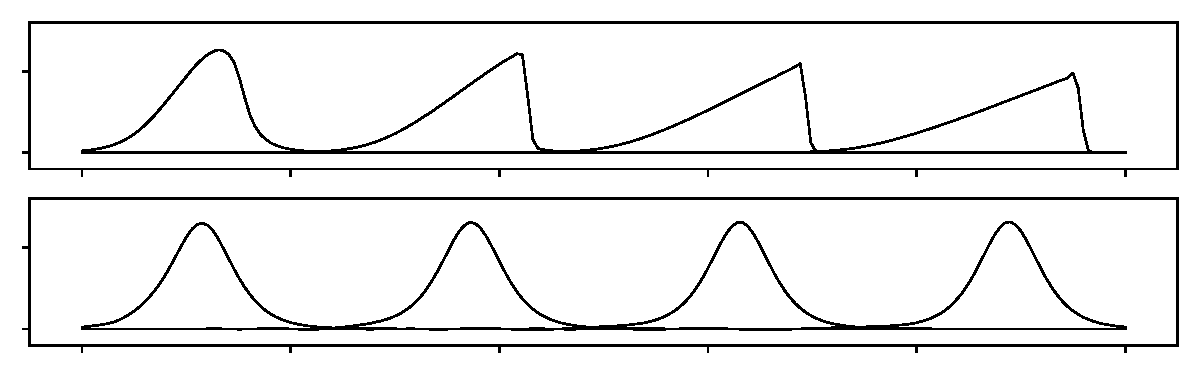
\includegraphics[width=.95\textwidth]{img/eq/boussinesq_dispersion.pdf}
    \caption{Boussinesq equations. Snapshots of a wave propagation. Top: Amplitude dispersion. Bottom: Frequency dispersion}
    \label{boussinesq_dispersion}
\end{figure}


In practice, this phenomenon does not happen. From linear wave theory we know that the celerity depends not only on the water depth, but also on the wavenumber $k=2\pi/\lambda$. This is known as frequency dispersion and this mechanism is missing on the Saint-Venant equations. The introduction of some extra terms leads to the Boussinesq equations, which model the frequency dispersion. Once the frequency dispersion is included, classical soliton waves can be obtained. In a soliton wave, breaking never occurs during the propagation, since the non linear terms are in equilibrium with dispersive terms.



%%%%%%%%%%%%%%%%%%%%%%%%%%%%%%%%%%%%
%%%%%%%%%%%%%%%%%%%%%%%%%%%%%%%%%%%%



\subsection{Derivation of the modified Boussinesq equations}

There are different ways to derive the Boussinesq equations with slightly different results. Nwogu presented a general framework in \cite{nwogu1993}. A three dimensional wave field with free surface elevation $\eta(x_1, x_2, t)$ and water depth at rest $H(x_1, x_2)$ is considered. The fluid is governed by the Navier-Stokes equations but the shallow water assumptions are modified. The fluid is assumed to be incompressible and the flow is assumed to be irrotational. As in the shallow water equations, the vertical velocity is considered to be small, but the vertical acceleration is not negligible. The nonlinearity and dispersion ratios (\ref{nonlin_disp_ratios}) are assumed to be small. The last difference between the shallow water equations and the Boussinesq consist in considering the horizontal velocity at a specified water depth instead of the mean value.

\begin{figure}
    \centering
    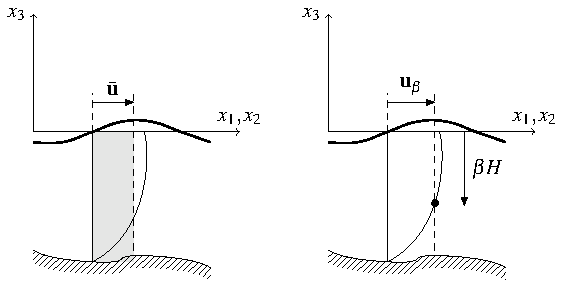
\includegraphics[width=.9\textwidth]{img/eq/velocity_beta.pdf}
    \caption{The modified Boussinesq equations consider the velocity at an arbitrary depth $\beta H$ instead of the mean velocity}
\end{figure}

Finally, the fluid at the free surface has to satisfy a dynamic and kinematic boundary conditions. At the bottom, the fluid has to satisfy a kinematic boundary condition.

\begin{equation}\label{dyn_kyn_bc}
\begin{aligned}
p &= 0 \ , \quad &&\text{at } x_3=\eta \\
u_3 &= \pder{\eta}{t} + u_1 \pder{\eta}{x_1}  + u_2 \pder{\eta}{x_2} \ , \quad &&\text{at } x_3=\eta \\
u_3 &= -u_1 \pder{H}{x_1} -u_2 \pder{H}{x_2} \ , \quad &&\text{at } x_3=-H
\end{aligned}
\end{equation}

Then, the continuity and momentum equations are integrated from the bottom to the free surface and applying the boundary conditions (\ref{dyn_kyn_bc}). Since the average horizontal velocity has been substituted by the velocity at a certain depth, the vertical profile of the velocities must be known. The key of the Boussinesq equations consist in finding an assumption which preserves the the effect of the frequency dispersion. The horizontal velocities $\mathbb{u}=(u_1, u_2)$ are expanded in Taylor series from the seabed ($x_3=-H$),
\begin{multline} \label{seabed_taylor_expansion}
    \mathbf{u}(x_1,x_2,x_3,t) = \mathbf{u}(x_1,x_2,-H,t) + (z+H)\mathbf{u}_3(x_1,x_2,-H,t) \\ + \sfrac{1}{2}(z+H)^2\mathbf{u}_{3,3}(x_1,x_2,-H,t) + \dots
\end{multline}
where the $3$ subscript denotes differentiation with respect to $x_3$.
Finally, the equations are evaluated at an arbitrary depth $x_3=\beta H$ and the set of Boussinesq-type equations are:

\begin{subequations} \label{bsq_eq}
\begin{equation} \label{bsq_eq_mom}
    \pder{\mathbf{u}_\beta}{t} + \nabla \eta + (\mathbf{u}_\beta \cdot \nabla) \mathbf{u}_\beta + \mathbf{J}_u = \mathbf{0}
\end{equation}
\begin{equation} \label{bsq_eq_mass}
    \pder{\eta}{t} + \nabla \cdot \left((H+\eta)\mathbf{u}_\beta\right) + \nabla \cdot \mathbf{J}_\eta = 0
\end{equation}
\end{subequations}
where the auxiliary fields $\mathbf{J}_\eta$ and $\mathbf{J}_u$ introduce the dispersive mechanism and are defined according to the following expressions
\begin{subequations} \label{bsq_eq_auxiliary_J}
\begin{equation}
    {J}_\eta =
        C_1 H^3 \nabla \nabla \cdot \mathbf{u}_\beta +
        C_3 H^2 \nabla \nabla \cdot (H \mathbf{u}_\beta) 
\end{equation}
\begin{equation}
    {J}_u =
        C_2 H^2 \nabla \nabla \cdot \pder{\mathbf{u}_\beta}{t} +
        C_4 H   \nabla \nabla \cdot \pder{(H \mathbf{u}_\beta)}{t} 
\end{equation}
\end{subequations}
and the $C_i$ constants depend on the choice of $\beta$
\begin{equation} \label{bsq_eq_C_constants}
    C_1=\frac{1}{2}\left(\beta^2-\frac{1}{3}\right)\ ,
    C_2=\frac{\beta^2}{2}\ ,
    C_3=\beta + \frac{1}{2}\ ,
    C_4=\beta
\end{equation}



%%%%%%%%%%%%%%%%%%%%%%%%%%%%%%%%%%%%%%%%
%%%%%%%%%%%%%%%%%%%%%%%%%%%%%%%%%%%%%%%%



\subsection{Dispersion properties and range of applicability}

This equations present as a free parameter $\beta$ the relative elevation at which the velocity is evaluated. Its value goes from $-1$ at the seabed, to $0$ at the free surface. Since the equations are an approximation of the fully dispersive and nonlinear problem, the parameter $\beta$ is chosen to minimize the errors introduced by the approximation.
In fact, the original Boussinesq equations does no present any dispersive term in the mass balance equation (\ref{bsq_eq_mass}) and correspond to a specific choice of $\beta$.

The parameter $\beta$ is fixed to $-0.531$ in \cite{nwogu1993}. This value has been obtained reducing the equations (\ref{bsq_eq}) to one dimension and flat bottom. Then, a trial function of small amplitude periodic wave of the type
\begin{equation*}
    \eta = a_0 \exp(i(kx-\omega t)) \ , \quad u_\beta = u_0 \exp(i(kx-\omega t))
\end{equation*}
is substituted into (\ref{bsq_eq_mass}) and (\ref{bsq_eq_mom}). After some algebraic manipulation the following expression for the phase speed is obtained:
\begin{equation}
c^2 = \frac{\omega^2}{k^2} = gh
    \left(\frac{
        1-\left(\frac{1}{2}\beta^2 + \beta + \frac{1}{3}\right)(kh)^2
    }{
        1-\left(\frac{1}{2}\beta^2 + \beta\right)(kh)^2
    }\right)
\end{equation}
The relation between the frequency and the wavelength is also known as \emph{dispersion relation}.
By the other hand, the dispersion relation given by the Linear wave theory or Airy theory is given by
\begin{equation}
c^2 = gh \frac{\tanh kh}{kh}
\end{equation}

Finally, the value of $\beta$ has been chosen to minimize the error at the range of applicability. Some other classical values of beta were obtained in \cite{madsen1991,murray1989}. Figure \ref{phase_speed_beta} shows the sensitivity of the phase speed depending on the parameter $\beta$. The shallow water equations, which drop the dispersive terms of equations (\ref{bsq_eq}) are only valid for the shallow water regime ($kh<0.3$). Fixing the free parameter $\beta=-0.531$ extend the range of applicability of the Boussinesq equations to intermediate depths ($kh<3$).

\begin{figure}
    \centering
    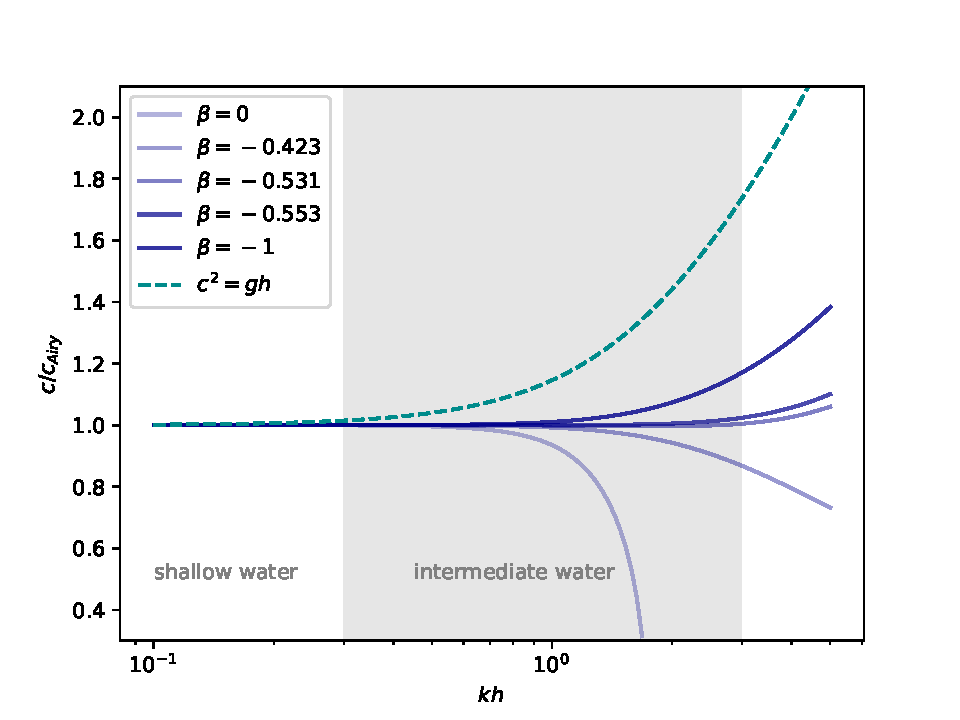
\includegraphics[width=.8\textwidth]{img/eq/dispersion_beta.pdf}
    \caption{Comparison of normalized phase speeds of the Boussinesq modified equations for different values of $\beta$}
    \label{phase_speed_beta}
\end{figure}

According to \cite{ursell1953} the nonlinearity and dispersion parameters $\epsilon$ and $\mu$ can be used for an alternative classification:

\begin{description}
    \item[$\epsilon \ll \mu$]  This configuration correspond to the case where frequency dispersion dominates the problem and linear or Airy theory must be used.
    \item[$\epsilon \sim \mu$] In this case frequency and amplitude dispersion are of the same magnitude and the Boussinesq approximation can be used.
    \item[$\epsilon \gg \mu$] In this situation the amplitude dispersion dominates the problem and the wave will eventually break. This can be simulated using the Saint-Venant or shallow water equations. Since the vertical velocity is assumed negligible, the pressure distribution is assumed to be constant.
\end{description}



%%%%%%%%%%%%%%%%%%%%%%%%%%%%%%%%%%%%%%%%%%%
%%%%%%%%%%%%%%%%%%%%%%%%%%%%%%%%%%%%%%%%%%%



\subsection{Boundary conditions}
\label{equations_bsq_bc}


The boundary conditions presented in section \ref{equations_sw_bc} are applicable to the Boussinesq equations.
However, since the oscillatory behavior is usually prevalent over the convective phenomenon, the boundary conditions are slightly different, both from the physical and the numerical point of view.
The three types of boundary conditions considered for the Boussinesq problems, inflow $\Gamma_I$, reflecting $\Gamma_R$ and absorbing $\Gamma_A$ boundaries have a direct equivalence respectively with the inflow $\Gamma_I$, solid $\Gamma_S$ and outflow $\Gamma_O$ boundaries stated in section \ref{equations_sw_bc}. Those subdomains are such that $\Gamma_I \cup \Gamma_R \cup \Gamma_A = \partial \Omega$, being $\partial\Omega$ the boundary of the domain.

\paragraph{Inflow boundary} Both free surface and velocity are known at $\Gamma_I$. Typically it is used to impose a wave generator. Since the wave amplitude is known, the horizontal velocity can be obtained using linear wave theory.

\paragraph{Reflecting boundary} No fluid should pass through an impermeable wall. This implies imposing the normal component of the velocity to be zero.
\begin{equation*}
    \bar{\mathbf{u}} \cdot \mathbf{n} = 0 \quad \text{on} \ \Gamma_R
\end{equation*}
Following Woo and Liu \cite{woo2004a}, the above relation must be rewritten in terms of $\mathbf{u}_\beta$ and the velocities are related as
\begin{equation*}
    \bar{\mathbf{u}} = \mathbf{u}_\beta + H^{-1} \mathbf{J}_\eta
\end{equation*}
Hence, the complete formulation of a reflective boundary is
\begin{equation}
    \bar{\mathbf{u}}_\beta \cdot \mathbf{n} = 0 \quad
    \mathbf{J}_\eta \cdot \mathbf{n} = 0 \quad
    \text{on} \ \Gamma_R
\end{equation}

\paragraph{Absorbing boundary} An outgoing wave should not return to the computational domain through $\Gamma_A$. A practical implementation of the absorbing boundaries are the sponge layers \cite{israeli1981, wei1995} and will be explained in section \ref{eulerian_bsq_absorbing}






%\include{chapters/chapter3}
%\include{chapters/chapter4}
%\include{chapters/chapter5}

%----------------------------------------------------------------------------------------
%	THESIS CONTENT - APPENDICES
%----------------------------------------------------------------------------------------

\appendix % Cue to tell LaTeX that the following "chapters" are Appendices

% Include the appendices of the thesis as separate files from the appendices folder

% Appendix Template

\chapter{Appendix Title Here} % Main appendix title

\label{AppendixX} % Change X to a consecutive letter; for referencing this appendix elsewhere, use \ref{AppendixX}

Write your Appendix content here.
%\include{appendices/appendixB}
%\include{appendices/appendixC}

%----------------------------------------------------------------------------------------
%	BIBLIOGRAPHY
%----------------------------------------------------------------------------------------

\printbibliography[heading=bibintoc]

%----------------------------------------------------------------------------------------

\end{document}  
